\documentclass[a4paper]{ctexart}  
\usepackage{graphicx,geometry}
\usepackage{pdfpages}
\usepackage[super,square]{natbib}%上标引用宏包

\geometry{left=2.0cm,right=2cm,top=2.45cm,bottom=2.45cm}
\bibliographystyle{unsrt}

\begin{document}  
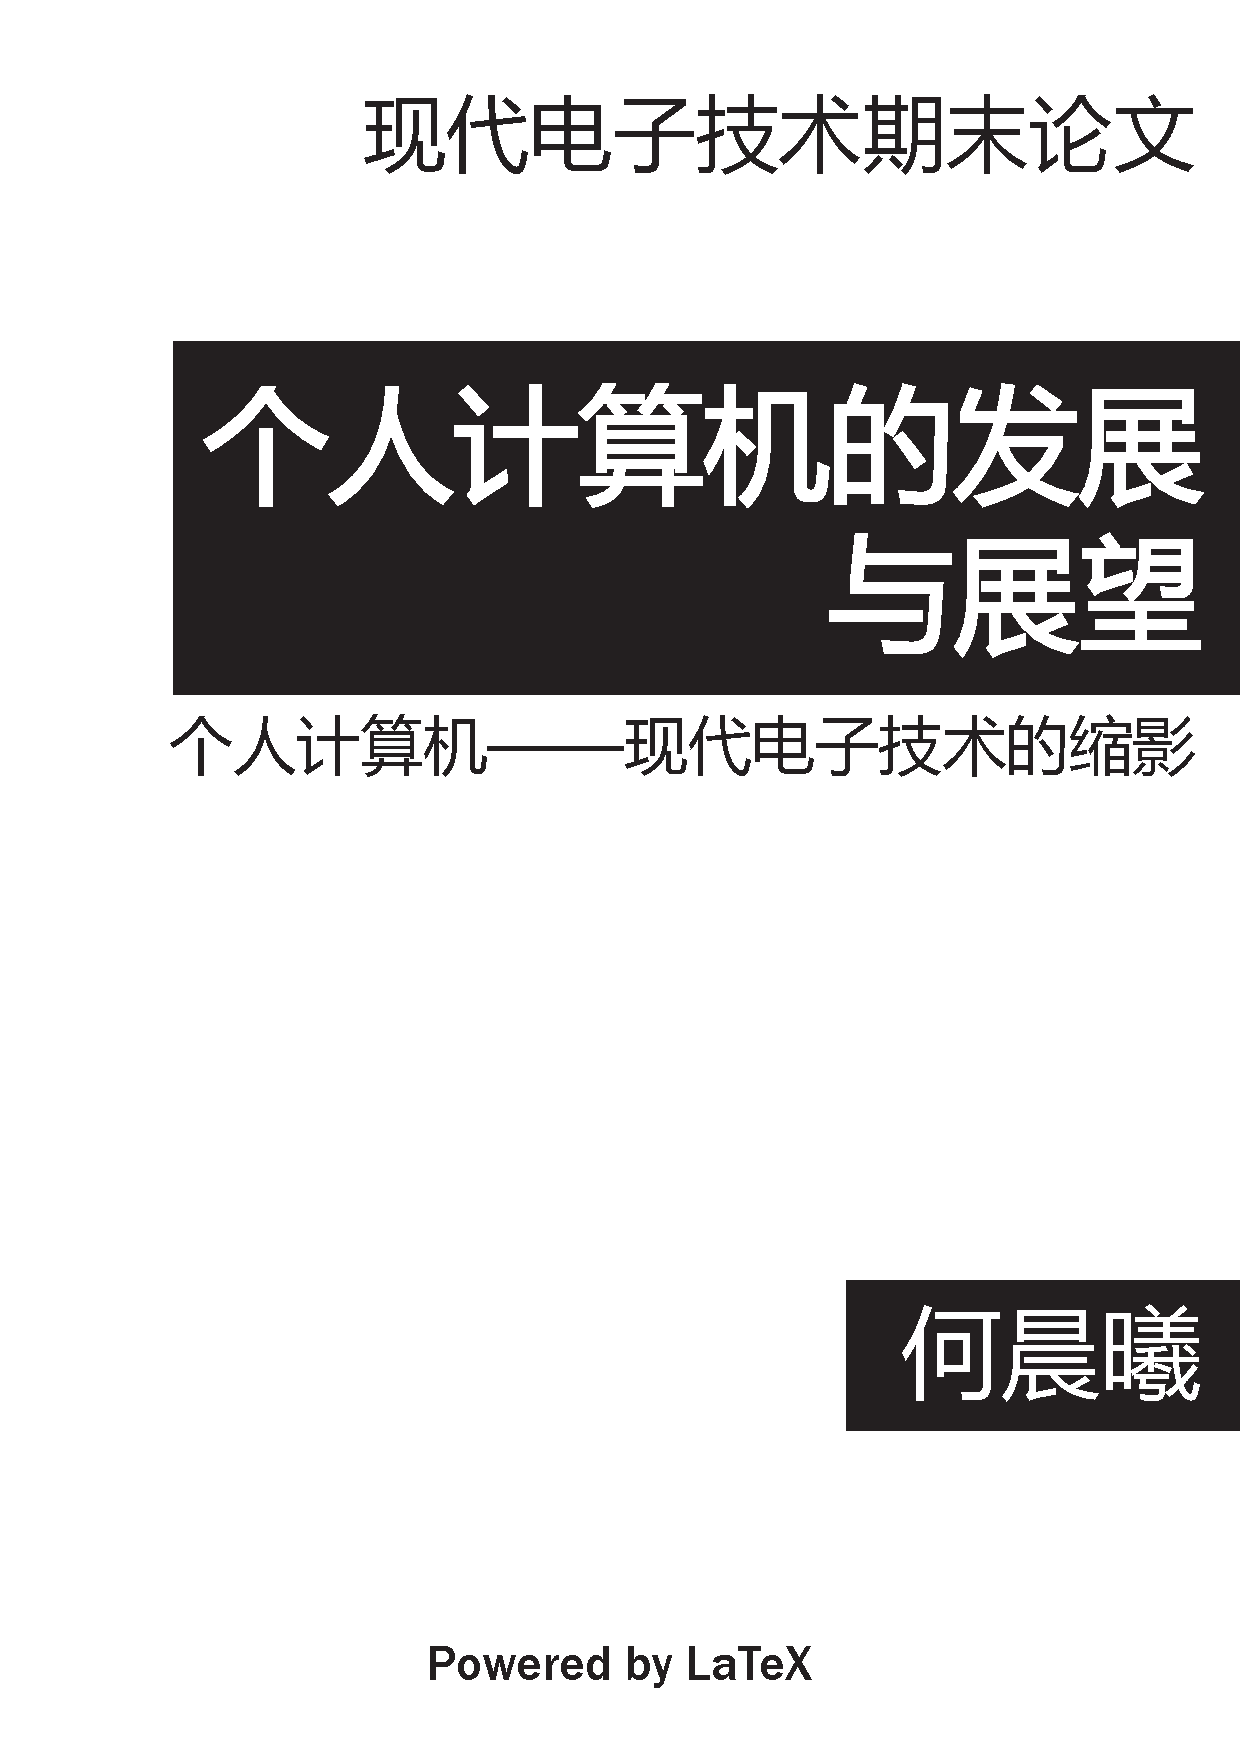
\includepdf[pages={1}]{pdf/cover.pdf} 

\tableofcontents%生成目录
\thispagestyle{empty}%目录页不显示页码
\newpage 

\setcounter{page}{1}%从下面开始编页码
\section{前言}
本节将对电子技术的发展做一个简单回顾,引出现代电子技术与个人计算机的话题。在电子技术的发展历程中有着一大批的伟大科学家,我毫不吝啬的使用了“伟大”这个词,因为正是由于他们的杰出贡献,才使得我们这个世界如此的缤纷多彩。
\subsection{电子技术的发展}
要讲清楚电子技术的发展,首先要先搞清楚,什么是电子技术。查询百科词条“电子技术”,电子技术是根据电子学的原理,运用电子元器件设计和制造某种特定功能的电路以解决实际问题的科学\footnote{来自百度百科}。所以电子技术的发展首先是电子学的发展。1895年汤姆逊(J.J.Thomson),用阴极射线的方法发现了电子,电子是一种基本粒子,是普通物质带负电的构成部分\cite{丹尼尔1977科学技术百科全书}。在电子被发现后,研究电子产生与运动的学科,即电子学,便诞生了。随后电子学又和无线电技术相结合,形成了我们今天的电子技术,在当今世界各个领域都离不开电子技术的应用\cite{刘伟平1999电子技术和光子技术的发展比较}。

首先推动电子技术的发展是人们对通信技术的需要。最早,人们靠人力来直接传递信息,著名的马拉松运动便是从传递军事信息由来的。我国古代则是使用烽火台来传递信息,但是表达的内容过于单一,且传递速度还是太慢了。在人们掌握电流的使用后,美国人莫尔斯发明了一种有线通信———电报机。随后电磁场的理论建立了起来,俄国人波波夫发明了世界上第一台无线电接收机,第二年,意大利人马可尼则是研制出第一台无线电发报机,无线电技术步入全新的时代。

电子技术的第二波推动力量则是电子器件的产生。首先就是真空电子管的发明,1904年由美国人费莱明
发明了真空二极管,1906年,美国人弗雷斯特发明了真空三极管。随后便是半导体材料的发现,美国贝尔实验室的肖克莱、巴丁、布拉顿等人经过多次试验,终于在1947年制造出世界上第一个晶体管,电子技术有进一步的迈进\cite{陈哲2004电子技术的发展}。二极管的特性是单向导电性,加正向电压时,电流很大,加反向电压时,电流很小,理想二极管的反向电流为0,三极管的特性是电流放大\cite{童诗白2001模拟电子技术基础}。1958年,Jack Kilby和他的同事,在德州仪器的实验室里成功的实现了把电子器件集成到一块半导体材料上的构想, 他也因此获得了2000年的诺贝尔物理学奖,为现代信息技术奠定了基础,人类文明开始进入了电子技术的时代。
\subsection{现代电子技术与个人计算机}
个人计算机是伴随着现代电子技术发展而来的,更是现代电子技术的缩影。上个世纪六十年代时,人类发明了晶体管,电子技术开始发展并被应用于生产生活中,随着电子技术的快速发展和广泛使用,社会的生产率获得了极大的提高,国家经济的发展水平也随着电子技术的推广得到了很大的提高。随着社会进入到信息时代,电子计算机技术的广泛应用, 对当前人们的工作和生活产生了巨大的影响。现如今,电子技术被广泛的应用到各个方面,其中最重要的方面便是个人计算机\cite{卡丽比努尔·塔什铁木尔2015现代电子技术与计算机应用的探讨}
\clearpage
\section{现代电子技术的缩影——个人计算机}

\subsection{个人计算机的发展}
早期的计算机使用机器语言\footnote{本小节内容来自纪录片\emph{Triumph of the Nerds}的总结},并且不同的计算机还有着不同的机器语言,你给计算机的指令也必须是代码形式的,来告诉计算机该做什么。在早些年,通过拨动开关或是加载纸带来输入指令,这使得计算机非常难用。后来一个名叫Grace Hopper的美国海军军官解决了这个问题,她发明了一种使用英语单词的计算机语言,计算机自己能够把这些单词翻译成二级制代码。这个首创的计算机语言有一个很傻的名字——COBOL。后面的一些语言,像FORTRAN和BASIC才使得计算机一点点变得好用起来。
个人计算机的发展是伴随着处理器的发展而发展的。早期的计算机,使用的是真空管或电子管,后来电子管被晶体管取代,处理器的体积进一步被缩小。后来,集成电路的发展为个人计算机的发展注入了强劲的动力。一块小小的单晶硅就可以腐蚀上亿个晶体管。这就是个人计算机的秘密,这也是为什么硅谷称为硅谷而不是计算机谷或者其他的什么谷。
说到这里就不得不提到英特尔了,INTEL拥有一切,但是它没有抓住,抓住它的是
1975发布的Altair,它是世界上第一款个人电脑,但是它非常难用,比尔盖茨为它编写了第一个个人电脑语言,依然公众不关注。两个年轻的黑客,斯蒂芬和沃兹尼亚克在加州的车库里制造了苹果电脑来向他们的朋友”炫耀“,并且开公司,卖他们的电脑。到了1980,仅仅从加州的车库创建后四年,苹果就成为了世界上最大的PC制造商。当时整个计算机行业的产值高达数十亿美元。

计算机巨人IBM没有轻视它,它可以利用现有的科技组装出计算机的硬件,但却没有操作系统,于是IBM找到了比尔盖茨和Gary Lildall,Gary Lildall当时是有操作系统的,名叫CP/M,为IBM的PC开发操作系统。IBM由于不满Gary Lildall接待,转头找了微软,尽管当时微软并没有操作系统,但微软仍然承诺在极短的时间内提供IBM所要的东西。后来微软花了五万美元在他们镇上,从Tim Patterson手上买断了QDOS(Quick and Dirty Operating System),这就是后来的IBM PC-DOS。IBM在1981 8月发布了自己的PC。虽然只是现有技术的集成,但由于IBM的影响力,仍然引起了巨大的轰动,并且催生了一大批的模仿者——PC克隆机。但PC仍然很难使用,使用的是字符界面。需要一个革命来让它变得更加友好,这就是PC图形用户界面。
\begin{quote}
\kaishu 好的艺术家模仿,伟大的艺术家窃取                  \hfill               ——毕加索
\end{quote}

施乐(xerox)——就是那家复印机公司,希望能让办公室的计算机更加高效、更加愉快(非常的愉快)进行工作。1973的施乐/Alto计算机,有人可能会说它才是第一台PC,其实不是,因为它从来没销售过,而且它的组件就需要1万美元。1979年12月份,乔布斯特邀访问施乐,施乐一共向他演示三个东西,但是他只被第一个东西迷住了, 甚至没有真正的看到其他两个。那就是图形化的用户界面,乔布斯意识到,在未来某天所有的计算机都将用到这项技术,这就是个人计算的未来。回来后,他就是着手开发一款代号为Lisa的新PC,但出现了一些问题,他们不能让它工作,而且售价高达10000美元,这对普通PC买家来说太贵了。Apple Lisa在董事会看来就是乔布斯自己的“宠物项目”,所以就把他从这个项目中赶了出来。乔布斯在沉思了几个月之后,又接手了Jeff Raskin的一个项目,那就是Macintosh——以美国人最喜欢的苹果种类命名的一款电脑。乔布斯决心让它变成便宜版的Lisa。1983年初,苹果陷入了困境,那就是IBM发布的PC拥有各种软件,而IBM的软件不能在MAC上运行,Macintosh想要成功,就必须要有杀手级的应用。乔布斯找到了当时刚刚在IBM PC-DOS上大赚一笔的微软,和微软签了合同,为第一个Mac提供捆绑的应用程序,尽管苹果已经开发了这些应用程序,但是它们需要的内存太大。1984年1月24日,Macintosh发布了,Macintosh毫无疑问是世界上第一个带有真正图形用户界面的廉价个人电脑。但Macintosh并没有获得成功,一部分原因是它的售价高达2500美元,其中有1000美元是纯利润,乔布斯相信Macintosh是如此优秀,以至于让消费者心甘情愿为Macintosh的溢价付费。另一部分的原因是Macintosh上的应用还是相对于它竞争对手IBM太少了。后来苹果和Adobe达成了合作,Adobe的软件在Macintosh上的出色运行,也带来了一个全新的行业——桌面出版业。但桌面出版业的成功相对于乔布斯来说太迟了,Macintosh的销售惨淡,导致了1985年苹果董事会决议撤销他的经营大权,1985年九月17日离开了苹果。乔布斯离开苹果后的几年里,也确实成了苹果最赚钱的几年。

视线转回比尔盖茨。当他为Macintosh开发软件的时候,他就意识到,Macintosh的图像化用户界面,会对自己赚钱机器IBM PC-DOS造成巨大威胁。微软坚信必须把赌注压在图形用户界面。微软的团队多年来在没有“视窗”的办公大楼里,喝着喝不完的免费可乐来补充能量,开发着“视窗”(Windows)操作系统。1990年终于完成了Windows1.0的研发,最开始它相对于Macintosh可能是一个笑话,但盖茨是不屈不挠的,慢慢的它越来越好了。这让苹果很担心,他们认为Windows是复制Macintosh上的功能,所以最后他们起诉了微软,长达6年的诉讼最后以苹果的败诉而告终,微软的Windows也在这六年内占据了压倒性的市场份额。至此个人计算机在20世纪的故事暂时结束了,但新千年的故事还在继续……
\subsection{个人计算机的展望}
计算机系统包括两大方面,一是软件、二是硬件。软件的核心便是操作系统了,从上个世纪60年底到现在涌现了许许多多的操作系统,包括著名的Unix、Linux、Windows等等,计算机操纵系统便是对计算机硬件的控制,我们不妨对未来的计算机操作系统做一些展望。未来操作系统的展望随着计算机硬件的发展,操作系统的竞争也越来越激烈,所以未来计算机操作系统将会在智能、易用、安全、网络化、编程简易、视觉效果上有所突破。更智能:对硬件的需求更低,在系统启动的时间上,现在系统一般不超过20秒,以后可以在几秒内启动,系统可以自己纠错并对硬件故障给予排除。更易用:使用操作系统更加方便,没有限制,可以通过声音对机器进行控制,甚至直接用我们的大脑发出的电磁波来进行信息的输入和控制。更安全:现在病毒木马司空见惯,未来计算机操作系统的安全性是一个必须突破的课题,至少要摆脱现在被动防御的局面。网络化:早在九十年代初SUM公司就提出了著名的“网络就是计算机”的口号,很多人不能理解,而现在随着计算机和网络的发展,以后我们只需要一个浏览器和显示器就可以控制我们的计算机来为我们服务,所需要的应用软件都在一个非常巨大的服务器上,通过网络我们就可以访问。编程更简易:可以随心所欲的编写程序,达到你想得倒的结果。视觉更逼真:随着电影制作和游戏的开发,我们可以简单的观看3D电影。游戏画面更加绚丽逼真,而这一切只需要我们在一个计算机上就可以完成\cite{王波2011个人计算机操作系统的发展与展望}。

其次是硬件的展望,其中最主要的就是计算机的中央处理器。现在是2018年,目前的移动端CPU已经达到的7nm的制造工艺,如果回顾之前的一些预测,我们会发现一些有意思的东西。一篇2012年的论文展望未来的处理器发展,预测到:到2015年将采用17nm工艺,2020年将采用10nm工艺。同时预测,到2013年,片上可集成的晶体管数将超过88亿个,片上局部时钟频率将达到7.3GHz。处理器核数目也呈现出同摩尔定律相似的指数增长规律, 从2,4,8核增加到64核甚至更多,从多核处理器发展为众核处理器。设计复杂程度达到前所未有的高度,对验证技术提出了巨大的挑战\cite{郭阳2012片上多核处理器验证}。可以看到,我们目前的制造工艺基本符合之前的预测,甚至还有些超过当年的预测,摩尔定律依然满足,但是我们也应该看到,目前处理器的性能提升其实是非常少的,几年的Intel i5处理器和现在的i5相比,其实性能并没有落后多少,进步最大的其实只有功耗比。未来的处理器向向什么方向发展,我想首先是集成度的进一步增加,但随之而来的发热问题也要得到解决,而且目前的制造工艺也遇到了瓶颈,该如何突破纳米效应这一难题,也是未来的研究方向,处理器的发展可能也会暂时的缓慢发展。其次,由于集成度的增加,我们的个人计算机的体积可能会进一步减少,可穿戴计算机也可能是未来的研究热点。
\section{总结}
通过对电子技术的发展做了一个简单的回顾,引出了现代电子技术的集大成者——个人计算机。接着对上个世纪,个人计算机波澜壮阔的发展史进行简单的回顾。最后对未来的个人计算机的发展进行了展望,包括了我们的个人计算机操作系统和计算机处理器。
\clearpage
\bibliography{references}
\end{document}  
